\section*{Lagrangian Systems and the Principle of Least Action}

\begin{definition}[Lagrangian System]
	A \bld{Lagrangian system}\index{Lagrangian!system} is defined to be a tuple $(M,L)$ consisting of an object $M \in \mathsf{Diff}$ and a morphism $L \in \mathsf{Diff}(TM \times \mathbb{R},\mathbb{R})$, called a \bld{Lagrangian function}\index{Lagrangian!function}.
\end{definition}

\begin{definition}[Path Space]
	\label{def:path_space}
	Let $M \in \mathsf{Diff}$, $q_0,q_1 \in M$ and $t_0, t_1 \in \mathbb{R}$ with $t_0 \leq t_1$. Define the \bld{path space of $M$ connecting $(q_0,t_0)$ and $(q_1,t_1)$}\index{Path space} to be the set
	\begin{equation}
		\label{eq:path_space}
		\mathcal{P}(M)^{q_0,t_0}_{q_1,t_1} := \cbr[0]{\gamma \in \mathsf{Diff}(\intcc[0]{t_0,t_1},M) : \gamma(t_0) = q_0 \text{ and } \gamma(t_1) = q_1}.
			\end{equation}
\end{definition}

\begin{remark}
	For the sake of simplicity, we will just use the terminology \emph{path space} for $\mathcal{P}(M)^{q_0,t_0}_{q_1,t_1}$ and simply write $\mathcal{P}(M)$. We implicitely assume the conditions of definition \ref{def:path_space}, however.
\end{remark}

\begin{definition}[Variation]
	\label{def:variation}
	Let $\mathcal{P}(M)$ be a path space and $\gamma \in \mathcal{P}(M)$. A \bld{variation of $\gamma$}\index{Variation} is defined to be a morphism $\Gamma \in \mathsf{Diff}(\intcc[0]{t_0,t_1} \times \intcc[0]{-\varepsilon_0,\varepsilon_0},M)$ for some $\varepsilon_0 > 0$ and such that
	\begin{itemize}[wide=0pt]
		\item $\Gamma(t,0) = \gamma$ for all $t \in \intcc[0]{t_1,t_0}$.
		\item $\Gamma(t_0,\varepsilon) = q_0$ for all $\varepsilon \in \intcc[0]{-\varepsilon_0,\varepsilon_0}$.
		\item $\Gamma(t_1,\varepsilon) = q_1$ for all $\varepsilon \in \intcc[0]{-\varepsilon_0,\varepsilon_0}$.
	\end{itemize}
\end{definition}

\begin{remark}
	If $\Gamma$ is a variation of $\gamma \in \mathcal{P}(M)$, we write $\gamma_\varepsilon(-) := \Gamma(-,\varepsilon)$ for all $\varepsilon \in \intcc[0]{-\varepsilon_0,\varepsilon_0}$.
\end{remark}

\begin{example}[Perturbation of a Path along a Single Direction]
	Let $M \in \mathsf{Diff}$ of dimension $n$, $(U,\varphi)$ a chart and suppose that $\gamma$ is a path in $U$. With respect to this chart, we can write the coordinate representation of $\gamma$ as
	\begin{equation*}
		\gamma(t) = \del[1]{\gamma^1(t),\dots,\gamma^n(t)}
	\end{equation*}
	\noindent for any $t \in \intcc[0]{t_0,t_1}$. Let $f \in C^\infty_c\intoo[0]{t_0,t_1}$. Consider the family $\Gamma : \intcc[0]{t_0,t_1} \times \intcc[0]{-\varepsilon_0,\varepsilon_0} \to M$ defined by
	\begin{equation*}
		\Gamma(t,\varepsilon) := (\iota \circ \varphi^{-1})\del[1]{\gamma^1(t),\dots,\gamma^i(t) + \varepsilon f(t),\dots,\gamma^n(t)}
	\end{equation*}
	\noindent where $\iota : U \hookrightarrow M$ denotes inclusion and $\varepsilon_0 > 0$ is to be determined. By exercise \ref{ex:U_delta_neighbourhood}, there exists $\delta > 0$ such that
	\begin{equation*}
		U_\delta := \cbr[0]{x \in \mathbb{R}^n : \dist(x,\gamma(\intcc[0]{t_0,t_1})) < \delta} \subseteq \varphi(U).
	\end{equation*}
	Choose $\varepsilon_0 > 0$ such that $0 < \varepsilon_0 < \delta/\norm{f}_\infty$. Then in coordinates
	\begin{equation*}
		\dist\del[1]{\gamma_\varepsilon(t), \gamma(\intcc[0]{t_0,t_1})} \leq \abs[0]{\gamma_\varepsilon(t) - \gamma(t)} = \abs{\varepsilon} \norm{f}_\infty \leq \varepsilon_0 \norm{f}_\infty < \delta 
	\end{equation*}
	\noindent for all $t \in \intcc[0]{t_0,t_1}$. Hence $\gamma_\varepsilon(t) \in U_\delta$ and thus $\gamma_\varepsilon(t) \in \varphi(U)$. Therefore, $\Gamma$ is indeed well-defined. Moreover, it is easy to show that the properties of definition \ref{def:variation} holds, therefore, $\Gamma$ is a variation of $\gamma$. In fact, this example shows, that any path $\gamma$ contained in a single chart admits infinitely many variations. An example of such a variation is shown in figure \ref{fig:variation}.

	\begin{figure}[h!tb]
		\centering
		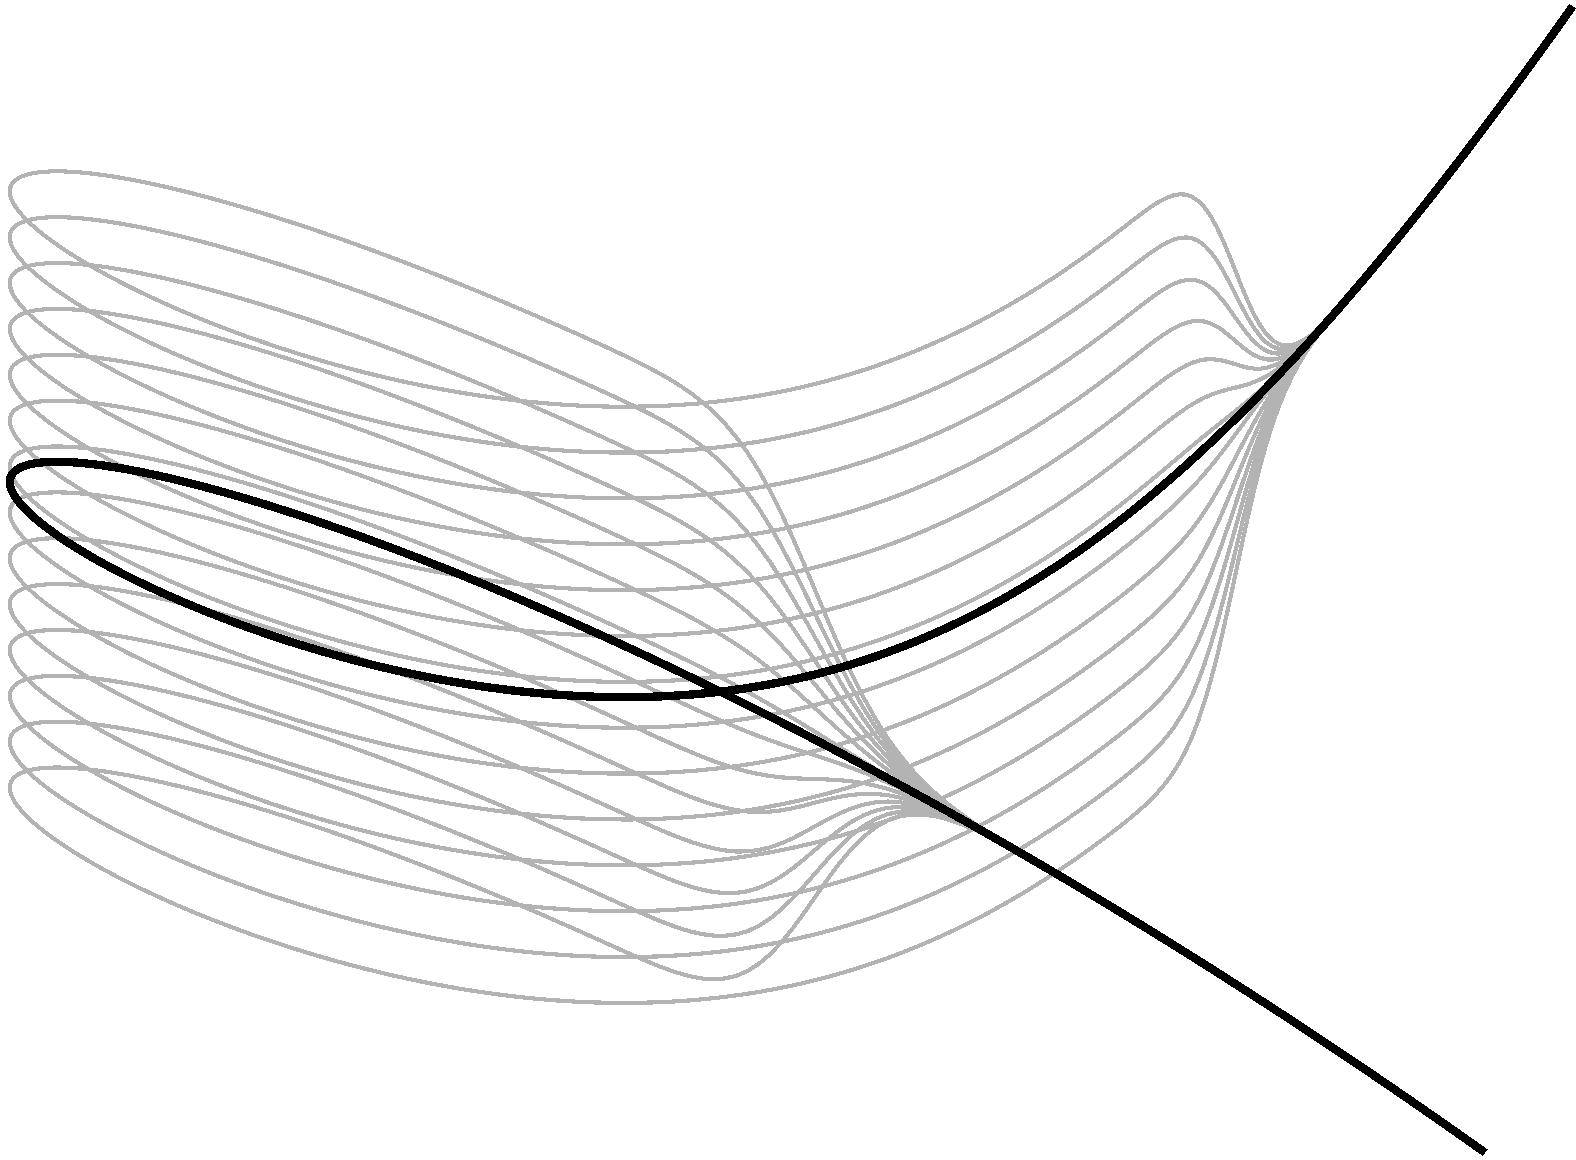
\includegraphics[width = .7\textwidth]{variation.jpg}
		\caption{Example of a variation along the second coordinate using a smooth bump function as in \cite[42]{lee:smooth_manifolds:2013}.}
		\label{fig:variation}
	\end{figure}
\end{example}

\begin{exercise}
	\label{ex:U_delta_neighbourhood}
	Let $U \subseteq \mathbb{R}^n$ open and $A \subseteq U$ closed. Then there exists $\delta > 0$ such that
	\begin{equation*}
		U_\delta := \cbr[0]{x \in \mathbb{R}^n : \dist(x,A) < \delta} \subseteq U.
	\end{equation*}
\end{exercise}

\begin{definition}[Action Functional]
	Let $(M,L)$ be a Lagrangian system and $\mathcal{P}(M)$ be a path space. The morphism $S : \mathcal{P}(M) \to \mathbb{R}$ defined by
	\begin{equation*}
		S(\gamma) := \int_{t_0}^{t_1} L(\gamma(t),\dot{\gamma}(t),t) dt
	\end{equation*}
	\noindent is called the \bld{action functional}\index{Action functional}.
\end{definition}

\begin{axiom}[Hamilton's Principle of Least Action]\index{Hamilton!'s principle of least action}
	Let $(M,L)$ be a Lagrangian system and $\mathcal{P}(M)$ be a path space. A path $\gamma \in \mathsf{Diff}(\intcc[0]{t_0,t_1},M)$ describes a motion of $(M,L)$ between $(q_0,t_0)$ and $(q_1,t_1)$ if and only if 
	\begin{equation}
		\frac{d}{d\varepsilon}\bigg\vert_{\varepsilon = 0} S(\gamma_\varepsilon) = 0
	\end{equation}
	\noindent for all variations $\gamma_\varepsilon$ of $\gamma$.
\end{axiom}

\begin{theorem}[Euler-Lagrange Equations]
	\label{thm:EL_equations}
	Let $(M,L)$ be a Lagrangian system. A path $\gamma \in \mathsf{Diff}(\intcc[0]{t_0,t_1},M)$ describes a motion of $(M,L)$ between $(q_0,t_0)$ and $(q_1,t_1)$ if and only if with respect to any chart $(U,q^i)$
	\begin{equation}
		\label{eq:EL_equations}
		\pd{L}{q}\del[1]{\gamma(t),\dot{\gamma}(t),t} - \frac{d}{dt} \pd{L}{\dot{q}}\del[1]{\gamma(t),\dot{\gamma}(t),t} = 0
	\end{equation}
	\noindent holds, where $(q,\dot{q})$ denotes the standard coordinates on $TM$. The system of equations \textup{(}\ref{eq:EL_equations}\textup{)} is referred to as the \bld{Euler-Lagrange equations}\index{Euler-Lagrange equations}.
\end{theorem}

\begin{proof}
	The proof is divided into three steps.
	\begin{enumerate}[label = \textit{Step} \arabic*:, wide = 0pt]
		\item \textit{Suppose that the extremal $\gamma$ is contained in a chart $(U,q^i)$.} 
	\end{enumerate}
\end{proof}
